% 
% (c) Copyright 2016 Tabea Mendez
% 
% This source is free: you can redistribute it and/or modify
% it under the terms of the GNU General Public License as published by
% the Free Software Foundation, either version 3 of the License, or
% (at your option) any later version.
% 
% This source is distributed in the hope that it will be useful,
% but WITHOUT ANY WARRANTY; without even the implied warranty of
% MERCHANTABILITY or FITNESS FOR A PARTICULAR PURPOSE.  See the
% GNU General Public License for more details.
% 
% You should have received a copy of the GNU General Public License
% along with this source.  If not, see <http://www.gnu.org/licenses/>.
%
%%%%%%%%%%%%%%%%%%%%%%%%%%%%%%%%%%%%%%%%%%%%%%%%%%%%%%%%%%%%%%%%%%%%%%%%%%%%%%


Die Fenster-Methode ist eine sehr simple Methode um FIR-Filter zu designen.
\begin{itemize}
 \item Der ideale Frequenzgang $D(\omega)$ wird in eine unendlich lange Impulsantwort $d(k)$ umgerechnet.\\[0.2cm]
 \fcolorbox{CadetRed}{white}{$D(\omega) = \mysum{k=-\infty}{\infty}{d(k)\,\e^{-j\omega k}}\qquad\Leftrightarrow\qquad d(k) = \dfrac{1}{2\pi}\myint{-\pi}{\pi}{D(\omega)\,\e^{j\omega k}}{\omega}$}\\[-1.65cm]
\end{itemize}
\begin{minipage}{0.7\textwidth}
	\begin{itemize}
	 \item Die unendlich lange Impulsantwort $d(k)$ wird symmetrisch mittels eines Fensters $w(n)$ bei $\pm M$ begrenzt. Dadurch ist die totale Anzahl Filterkoeffizienten ungerade. $\qquad$
	 \fcolorbox{CadetRed}{white}{$N = 2 M+1$}\\[0.2cm]
	 \fcolorbox{CadetRed}{white}{$\widehat D(\omega) = \mysum{k=-M}{M}{d(k)\,\e^{-j\omega k}}\qquad\Leftrightarrow\qquad d(k) = \dfrac{1}{2\pi}\myint{-\pi}{\pi}{D(\omega)\,\e^{j\omega k}}{\omega} \qquad -M\leq k \leq M$}
	\end{itemize}
\end{minipage}
\begin{minipage}{0.02\textwidth}$ $\end{minipage}
\begin{minipage}{0.28\textwidth}
	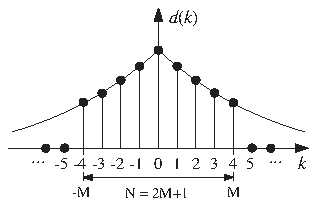
\includegraphics[width = \textwidth]{pic/FensterFIRFilter.pdf}\\[2.7cm]
\end{minipage}\\[-1.8cm]
\begin{itemize}
 \item Damit das FIR-Filter $h(n)$ kausal wird, muss die begrenzte Impuls-\\antwort $d(k)$ noch um $M$ Samples verzögert werden.\\[0.2cm]
 \fcolorbox{CadetRed}{white}{$ H(\omega) = \e^{-j\omega M} \,\widehat D(\omega) \qquad\Leftrightarrow\qquad  h(n) = d(n-M)\qquad n = 0,1,...,N-1$}\\[-0.25cm]
 \item Diese Verzögerung um $M$ Samples resultiert in einem linearphasigen Filter.
 \item Die Fenster-Methode ist sehr gut geeignet für einfache Frequenzgänge wie die folgender Filter.\\
\end{itemize}

\begin{tabularx}{\textwidth}{|>{\centering\arraybackslash}p{4.5cm}|>{\centering\arraybackslash}p{8.7cm}|X|}
 \hline&&\\[-0.3cm]
	\textbf{Filter} & \textbf{Frequenzgang $D(\omega)$ und Impulsantwort $d(k)$}& \textbf{Eigenschaften}\\[0.1cm]
 \hline&&\\[-0.2cm]
	Tiefpass &
	\multirow{2}{*}{$\begin{array}{c}\text{\fcolorbox{CadetRed}{white}{$D(\omega) = \begin{cases}1,&-\omega_c\leq\omega\leq\omega_c\\ 0,& \text{sonst}\end{cases} $}}\\[0.7cm]
	\text{\fcolorbox{CadetRed}{white}{$d(k) = \dfrac{\sin(\omega_ck)}{\pi k} $}}\end{array}$}&
	\multirow{8}{*}{$\begin{array}{l}
	\!\!\!\text{Der Frequenzgang ist:}\\\text{- reell}\\\text{- gerade}\\\text{- symmetrisch}\\[0.4cm]
	\!\!\!\text{Die Impulsantwort ist:}\\\text{- zweiseitig (akausal)}\\\text{- unendlich lang}\\\text{- reell}\\\text{- gerade}\\\text{- symmetrisch}\end{array}$}\\
	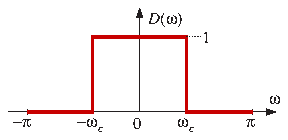
\includegraphics[width = 0.25\textwidth]{pic/tiefpass.pdf}&
	&
	\\[0.15cm]
 \cline{1-2}&&\\[-0.2cm]
	Hochpass &\multirow{2}{*}{$\begin{array}{c}\text{\fcolorbox{CadetRed}{white}{$D(\omega) = \begin{cases}0,&-\omega_c\leq\omega\leq\omega_c\\ 1,& \text{sonst}\end{cases} $}}\\[0.7cm]
	\text{\fcolorbox{CadetRed}{white}{$d(k) = \delta(k) - \dfrac{\sin(\omega_ck)}{\pi k} $}}\end{array}$}&\\
	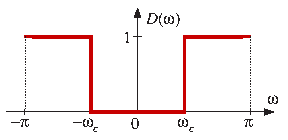
\includegraphics[width = 0.25\textwidth]{pic/hochpass.pdf}&
	&
	\\[0.15cm]
 \cline{1-2}&&\\[-0.2cm]
	Bandpass &\multirow{2}{*}{$\begin{array}{c}\text{\fcolorbox{CadetRed}{white}{$D(\omega) = \begin{cases}1,&-\omega_b\leq\omega\leq-\omega_a\;\;\cup\;\;\omega_a\leq\omega\leq\omega_b\\ 0,& \text{sonst}\end{cases} $}}\\[0.7cm]
	\text{\fcolorbox{CadetRed}{white}{$d(k) = \dfrac{\sin(\omega_bk)-\sin(\omega_ak)}{\pi k} $}}\end{array}$}&\\
	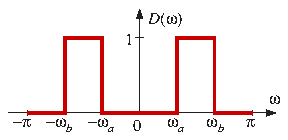
\includegraphics[width = 0.25\textwidth]{pic/bandpass.pdf}&
	&
	\\[0.15cm]
 \cline{1-2}&&\\[-0.2cm]
	Bandsperre &
	\multirow{2}{*}{$\begin{array}{c}\text{\fcolorbox{CadetRed}{white}{$D(\omega) = \begin{cases}0,&-\omega_b\leq\omega\leq-\omega_a\;\;\cup\;\;\omega_a\leq\omega\leq\omega_b\\ 1,& \text{sonst}\end{cases} $}}\\[0.7cm]
	\text{\fcolorbox{CadetRed}{white}{$d(k) = \delta(k) - \dfrac{\sin(\omega_bk)-\sin(\omega_ak)}{\pi k} $}}\end{array}$}&\\
	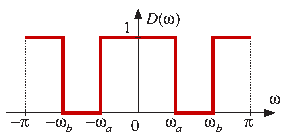
\includegraphics[width = 0.25\textwidth]{pic/bandsperre.pdf}&
	&
	\\[0.15cm]
 \hline
\end{tabularx}

\begin{tabularx}{\textwidth}{|>{\centering\arraybackslash}p{4.5cm}|>{\centering\arraybackslash}p{8.7cm}|X|}
 \hline&&\\[-0.3cm]
	\textbf{Filter} & \textbf{Frequenzgang $D(\omega)$ und Impulsantwort $d(k)$}& \textbf{Eigenschaften}\\[0.1cm]
 \hline&&\\[-0.2cm]
	Differenzierer &
	\multirow{2}{*}{$\begin{array}{c}\\[-0.2cm]\text{\fcolorbox{CadetRed}{white}{$D(\omega) = j\omega$}}\\[0.5cm]
	\text{\fcolorbox{CadetRed}{white}{$d(k) = \dfrac{\cos(\pi k)}{k} -  \dfrac{\sin(\pi k)}{\pi k^2} $}}\end{array}$}&
	\multirow{4}{*}{$\begin{array}{l}
	\!\!\!\text{Der Frequenzgang ist:}\\\text{- imaginär}\\\text{- ungerade}\\\text{- antisymmetrisch}\\[0.4cm]
	\!\!\!\text{Die Impulsantwort ist:}\\\text{- zweiseitig (akausal)}\\\text{- unendlich lang}\\\text{- reell}\\\text{- ungerade}\\\text{- antisymmetrisch}\end{array}$}\\
	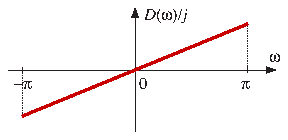
\includegraphics[width = 0.25\textwidth]{pic/differenzierer.pdf}&
	&
	\\[0.15cm]
 \cline{1-2}&&\\[-0.2cm]
	Hilbert-Transformator &\multirow{2}{*}{$\begin{array}{c}\\[-0.2cm]\text{\fcolorbox{CadetRed}{white}{$D(\omega) = -j\;\!\sgn(\omega)$}}\\[0.5cm]
	\text{\fcolorbox{CadetRed}{white}{$d(k) = \dfrac{1-\cos(\pi k)}{\pi k} $}}\end{array}$}&\\
	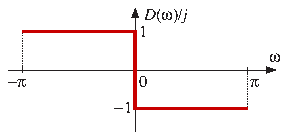
\includegraphics[width = 0.25\textwidth]{pic/hilberttransformator.pdf}&
	&
	\\[0.15cm]
 \hline
 
\end{tabularx}\\[0.1cm]
\FloatBarrier

	\section{Eigenschaft der linearen Phase}
		Wenn FIR-Filter mit der Fenster-Methode designt werden resultiert ein \textbf{linearphasiges Filter}, d.h. das Filter verzögert alle Frequenzen um genau gleich viele ($M$) Samples $\quad\Rightarrow\quad$ konstante Gruppenlaufzeit!\\[0.2cm]
		Dies kommt daher, dass ...
		\begin{itemize}
		 \item ... \textbf{symmetrische Impulsantworten keine Phase (Nullphasig) und damit keinen Delay haben.}
		 \item ... die Begrenzung einer symmetrischen/antisymmetrischen Impulsantwort die symmetrie/antisymmetrie beibehaltet und der Frequenzgang nach wie vor rein reell/imaginär ist. \\
		 \begin{danger}
		  Impulsantwort muss symmetrisch begrenzt werden, da sonst die Symmetrie und damit die\newline Linearphasigkeit aufgegeben wird.
		 \end{danger}
		 \item ... durch die eingeführte Zeitverzögerung (um das Filter kausal zu machen) aus dem nullphasigen Filter ein linearphasiges Filter wird.
		\end{itemize}$ $\\[-0.7cm]
		Die Linearphasigkeit ist in folgenden Formeln erkennbar wobei $\quad$\fcolorbox{black}{white}{$\beta(\omega) = \dfrac{1-\sgn(\widehat D(\omega))}{2} = \small\begin{cases}0,&\widehat D(\omega) > 0\\ 1,&\widehat D(\omega) < 0 \end{cases}$}\normalsize\\[-0.2cm]
		\textbf{Symmetrischer Fall (rein reell):}\\[0.2cm]
		$H(\omega)\; =\; \e^{-j\omega M} \,\widehat D(\omega) 
		\; =\; \e^{-j\omega M}\,\sgn(\widehat D(\omega))\, \big|\widehat D(\omega) \big|
		\; =\; \e^{-j\omega M}\,\e^{j\pi\beta(\omega)} \,\big|\widehat D(\omega) \big|\; =\; \underline{\e^{j(-\omega M+\pi\beta(\omega))}\,\big|\widehat D(\omega) \big|}$\\[0.2cm]
		$\;\;\Rightarrow\qquad$\fcolorbox{CadetRed}{white}{$\big|H(\omega) \big| = \big|\widehat D(\omega) \big|,\qquad \text{arg}H(\omega) \;\;=\;\; -\omega M\;\;+\underbrace{\pi\beta(\omega)}_{\text{Vorzeichenwechsel}}$}\\[0.2cm]
		\textbf{Antysymmetrischer Fall (rein imaginär):}\\[0.2cm]
		$\;\;\Rightarrow\qquad$\fcolorbox{CadetRed}{white}{$\big|H(\omega) \big| = \big|\widehat D(\omega) \big|,\qquad \text{arg}H(\omega) \;\;=\;\; -\omega M\;\;+\underbrace{\dfrac{\pi}{2}}_{\text{Offset für $j$}}+\underbrace{\pi\beta(\omega)}_{\text{Vorzeichenwechsel}}$}
	
	\section{Rechteck-Fenster}
		\begin{minipage}{0.5\textwidth}
			Das simpelste Fenster ist das Rechteck-Fenster\\[0.2cm] $\qquad$\fcolorbox{CadetRed}{white}{$w(n) =\begin{cases}1,&0\leq n\leq N-1\\0,&\text{sonst}\end{cases}$ }\\[0.4cm]
		\end{minipage}
		\begin{minipage}{0.5\textwidth}
			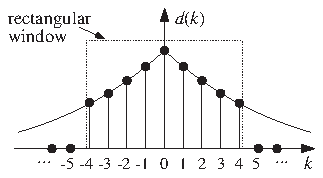
\includegraphics[width = 0.45\textwidth]{pic/rechteckFensterImpulsantwort.pdf}
			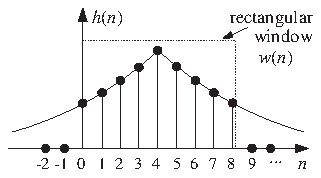
\includegraphics[width = 0.45\textwidth]{pic/rechteckFensterFilter.pdf}
		\end{minipage}
		Hierbei sind für das FIR-Filter-Design folgende Schritte notwendig:
		\begin{enumerate}
		 \item Wähle eine ungerade Länge $N = 2M+1$\\[-0.6cm]
		 \item Berechne die $N$ Koeffizienten von $d(k)$ mit $k = -M\leq k\leq M$. \textbf{Aufpassen bei $\bm{k=0}$!}\\[-0.6cm]
		 \item Verzögere $d(k)$ um $M$-Samples um ein kausales Filter zu erhalten $\quad $\fcolorbox{CadetRed}{white}{$h(n) = d(n-M)$}$\quad n=0,...,N-1$
		\end{enumerate}
\newpage
		
	\section{Hamming- und Hann-Fenster}
		Etwas komplexere Fenster sind das Hamming-Fenster und das Hann-Fenster.\\[0.2cm]
		\begin{minipage}{0.35\textwidth}
			Hamming-Fenster\\[0.2cm]
			\fcolorbox{CadetRed}{white}{$w(n) = 0.54-0.46\cos\left(\dfrac{2\pi n}{N-1}\right)$}\\[0.25cm]
			$n = 0,1,...,N-1$
		\end{minipage}
		\begin{minipage}{0.25\textwidth}
			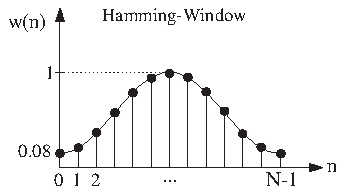
\includegraphics[width = \textwidth]{pic/hammingFenster.pdf}
		\end{minipage}\begin{minipage}{0.05\textwidth}$ $\end{minipage}
		\begin{minipage}{0.25\textwidth}
			Hann-Fenster\\[0.2cm]
			\fcolorbox{CadetRed}{white}{$w(n) = 0.5-0.5\cos\left(\dfrac{2\pi n}{N-1}\right)$}\\[0.25cm]
			$n = 0,1,...,N-1$
		\end{minipage}\\
		
		\begin{minipage}{0.7\textwidth}
		Hierbei sind für das FIR-Filter-Design folgende Schritte notwendig:\\[-0.2cm]
		\begin{enumerate}
		 \item Wähle eine ungerade Länge $N = 2M+1$\\[-0.3cm]
		 \item Berechne die $N$ Koeffizienten von $d(k)$ mit $k = -M\leq k\leq M$.\\ \textbf{Aufpassen bei $\bm{k=0}$!}\\[-0.3cm]
		 \item Verzögere $d(k)$ um $M$-Samples um ein kausales Filter zu erhalten und multipliziere die verzögerte Sequenz mit dem Fenster $w(n)$\\[0.1cm] 
		 $\quad $\fcolorbox{CadetRed}{white}{$h(n) = w(n)\,d(n-M)$}$\quad n=0,...,N-1$
		\end{enumerate}
		\end{minipage}\begin{minipage}{0.05\textwidth}$ $\end{minipage}
		\begin{minipage}{0.25\textwidth}
			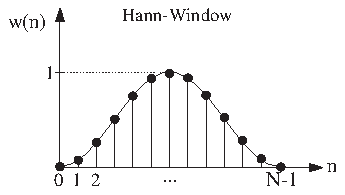
\includegraphics[width = \textwidth]{pic/hannFenster.pdf}\\[1.5cm]
		\end{minipage}
	\section{Frequenzgang der Filters mit dem Rechteck/Hamming-Fenster}
		\begin{itemize}
		 \item Beim Design mit der Fenster-Methode wird die verschobene Impulsantwort $d(n-M)$ mit einem Fenster multipliziert. Dies entspricht im Frequenzbereich einer Faltung.\\[0.2cm]
		 \fcolorbox{CadetRed}{white}{$h(n) = w(n)\,d(n-M)\qquad\Leftrightarrow\qquad H(\omega) = \dfrac{1}{2\pi}\myint{-\pi}{\pi}{W(\omega-\omega')\,\e^{-j\omega'M}\, D(\omega')}{\omega'}$}\\
		 \item Durch die Faltung werden die Rippel der Impulsantwort des Fensters $W(\omega)$ integriert, was zu Rippel und Überschwinger im Frequenzgang $H(\omega)$ führt.\\[0.1cm]
		 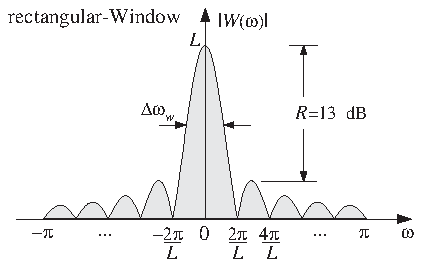
\includegraphics[width = 0.25\textwidth]{pic/spektrumRechteckFenster.pdf}$\quad$
		 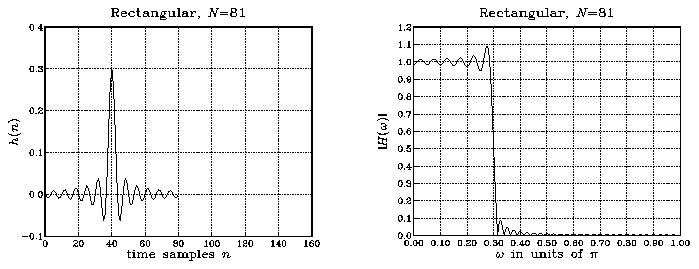
\includegraphics[width = 0.56\textwidth]{pic/spektrumRechteckFenster2.pdf}\\[0.1cm]
		 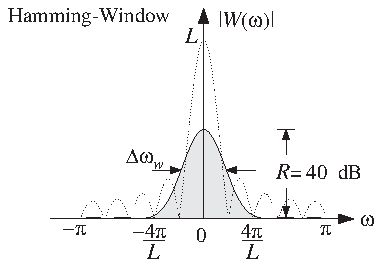
\includegraphics[width = 0.25\textwidth]{pic/spektrumHammingFenster.pdf}$\quad$
		 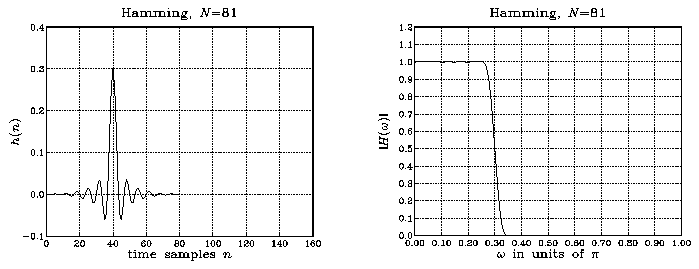
\includegraphics[width = 0.56\textwidth]{pic/spektrumHammingFenster2.pdf}
		 \item Der Frequenzgang $H(\omega)$ ist nur durch die Anzahl Samples $N$ beeinflussbar, dabei gilt:\\[0.1cm]
		 \fcolorbox{CadetRed}{white}{$N\Uparrow\qquad\Rightarrow\qquad \text{Übergangsbandbreite } \Delta\omega\Downarrow\quad\cap\quad $schnelleres abklingen der Überschwinger}
		 \item Die Höhe der Überschwinger ist fensterabhängig und damit bei fixen Fenstern immer gleich gross\\[0.1cm]
		 \begin{tabular}{|l|c|c|}
		  \hline&&\\[-0.35cm]
			& Höhe Überschwinger & Stoppband-Dämpfung\\[0.05cm]
		  \hline&&\\[-0.35cm]
			Rechteck-Fenster & $8.9\%$ & $-20\log(0.089) =21\db$\\[0.05cm]
		  \hline&&\\[-0.35cm]
			Hamming-Fenster & $0.2\%$& $-20\log(0.002)= 54\db$\\[0.05cm]
		  \hline
		 \end{tabular}
		 \item Der Frequenzgang hat bei $\omega_c$ immer die halbe Höhe$\qquad$\fcolorbox{CadetRed}{white}{$\big|H(\omega_c)\big| = 0.5$}
		\end{itemize}	
		
	\section{Kaiser-Fenster}
		\vspace*{-0.2cm}
		\begin{minipage}{0.52\textwidth}
			Das Kaiser-Fenster ist eine Fenster-Familie welches zwei Parameter hat. Dadurch können folgende zwei Dinge eingestellt werden.\\[-0.2cm]
			\begin{itemize}
			 \item Die Übergangsbandbreite $\Delta\omega$ über die Anzahl Samples $N$\\[-0.2cm]
			 \item Die Höhe der Überschwinger bzw. die Stoppband-Dämpfung $A_{stop}$ über den Parameter $\alpha$
			\end{itemize}
		\end{minipage}\begin{minipage}{0.03\textwidth}$ $\end{minipage}
		\begin{minipage}{0.45\textwidth}
		 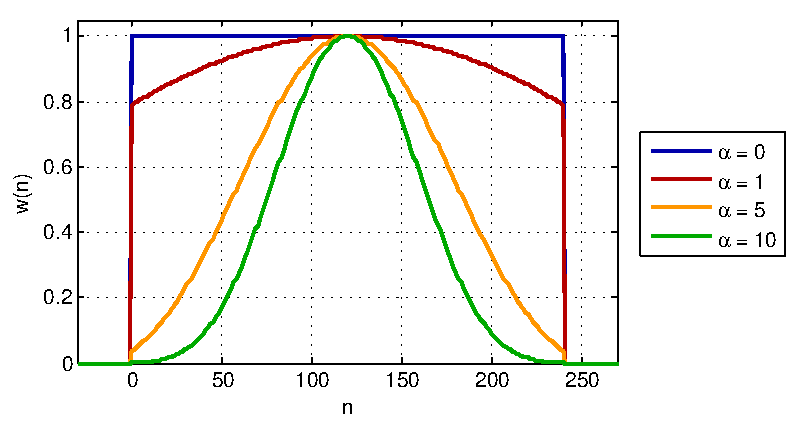
\includegraphics[width = \textwidth]{pic/KaiserFenster.pdf}
		\end{minipage}\\[0.1cm]
		\fcolorbox{CadetRed}{white}{$\begin{array}{lcl}w(n)&=&\dfrac{I_0(\alpha\sqrt{1-(n-M)^2/M^2})}{I_0(\alpha)}\\[0.5cm]& =& \dfrac{I_0(\alpha\sqrt{n(2M-n)}/M)}{I_0(\alpha)}\end{array}$}$\quad$
		$\begin{array}{l}n = 0,1,...,N-1\\[0.15cm] I_0(...):  \text{modifizierte Besselfunktion erster Gattung, 0-ter Ordnung.}\\[0.15cm] w(M) = 1 \;\;\text{und}\;\; w(0) = w(N-1) = 1/I_0(\alpha)\\[0.15cm] \alpha = 0\quad\Rightarrow\quad \text{Rechteck-Fenster}\end{array}$\\[0.4cm]
		\textbf{Für das FIR-Filter-Design mit Kaiser-Fenster müssen folgende Dinge gegeben sein:}\\[0.3cm]
		\begin{tabularx}{\textwidth}{>{\centering\arraybackslash}X|>{\centering\arraybackslash}X}
		 Tiefpass / Hochpass & Bandpass / Bandsperre\\[0.1cm]
		 \hline&\\[-0.3cm]
		 $\begin{array}{l}
		   \text{- Stopp- und Druchlass-Frequenz}\\[0.1cm]\qquad\text{\fcolorbox{CadetRed}{white}{$f_{stop}\;,\;f_{pass}$}}\\[0.3cm]\text{- Stopp- und Passband-Dämpfung}\\[0.1cm]\qquad\text{\fcolorbox{CadetRed}{white}{$A_{stop}\;,\;A_{pass}$}}
		  \end{array}$
		  & 
		  $\begin{array}{l}
		   \text{- Stopp- und Druchlass-Frequenz für beide Seiten}\\[0.1cm]\qquad\text{\fcolorbox{CadetRed}{white}{$f_{sa}\;,\;f_{pa}\;,\;f_{sb}\;,\;f_{pb}$}}\\[0.3cm]\text{- Stopp- und Passband-Dämpfung}\\[0.1cm]\qquad\text{\fcolorbox{CadetRed}{white}{$A_{stop}\;,\;A_{pass}$}}
		  \end{array}$\\[1.4cm]
		 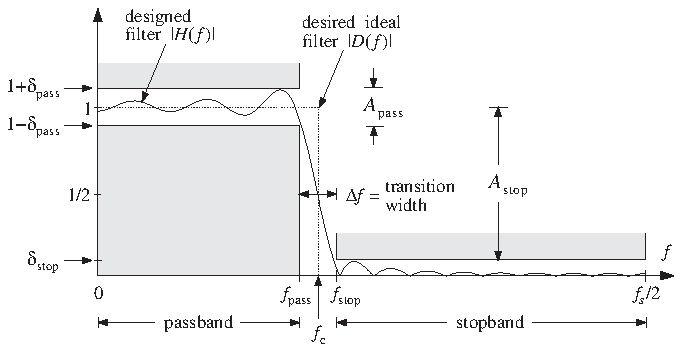
\includegraphics[width = 0.45\textwidth]{pic/kaiserTPHP.pdf}
		 & 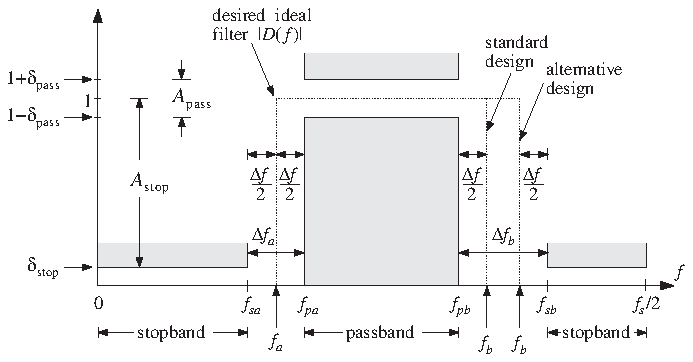
\includegraphics[width = 0.45\textwidth]{pic/kaiserBPBS.pdf}\\
		\hline
		\end{tabularx}\\[0.5cm]
		\textbf{Für das FIR-Filter-Design folgende Schritte notwendig:}\\[-0.4cm]
		\begin{enumerate}
		 \item Berechnung der Übergangsbandbreite $\Delta f$\\[0.2cm]
		 \begin{tabular}{c|c}
		 Tiefpass / Hochpass & Bandpass / Bandsperre\\[0.1cm]
		 \hline&\\[-0.3cm]
		 \text{$\quad$\fcolorbox{CadetRed}{white}{$\Delta f = \big|f_{stop} - f_{pass}\big| $}$\quad$} & \text{$\quad$\fcolorbox{CadetRed}{white}{$\Delta f = \min\{\Delta f_a,\Delta f_b\} $}$\quad$\fcolorbox{black}{white}{$\Delta f_a = \big|f_{pa} - f_{sa}\big|$}$\quad$\fcolorbox{black}{white}{$\Delta f_b = \big|f_{sb} - f_{pb}\big|$}$\quad$}\\
		 \end{tabular}\\
		 \item Berechnung der Eckfrequenz $f_c$ bzw. $f_a$ und $f_b$\\[0.2cm]
		 \begin{tabular}{c|c}
		 Tiefpass / Hochpass & Bandpass / Bandsperre\\[0.1cm]
		 \hline&\\[-0.3cm]
		 \text{$\quad$\fcolorbox{CadetRed}{white}{$f_c = \dfrac{1}{2}(f_{stop} + f_{pass})$}$\quad$} & \text{$\quad\begin{array}{lll}\text{Standard-Design:}& \text{\fcolorbox{CadetRed}{white}{$f_a = f_{pa}-\frac{1}{2}\Delta f $}}&\text{\fcolorbox{CadetRed}{white}{$f_b = f_{pb}+\frac{1}{2}\Delta f $}}\\[0.25cm]\text{Alternatives-Design:}& \text{\fcolorbox{CadetRed}{white}{$f_a = f_{sa}+\frac{1}{2}\Delta f $}}&\text{\fcolorbox{CadetRed}{white}{$f_b = f_{sb}-\frac{1}{2}\Delta f $}}\\\end{array}\quad$}\\
		 \end{tabular}\\
		  \item Berechnung der digitalen Eckfrequenz $\omega_c$ bzw. $\omega_a$ und $\omega_b$\\[0.2cm]
		 \begin{tabular}{c|c}
		 Tiefpass / Hochpass & Bandpass / Bandsperre\\[0.1cm]
		 \hline&\\[-0.3cm]
		 \text{$\quad$\fcolorbox{CadetRed}{white}{$\omega_c = \dfrac{2\pi f_c}{f_s}$}$\quad$} & \text{$\quad$\fcolorbox{CadetRed}{white}{$\omega_a = \dfrac{2\pi f_a}{f_s}$}$\qquad$\fcolorbox{CadetRed}{white}{$\omega_b = \dfrac{2\pi f_b}{f_s}$}$\quad$}\\
		 \end{tabular}\\
		 \item Berechnung der Stopp- und Passband-Dämpfung $\delta_{stop}$ und $\delta_{pass}$\\[0.2cm]
		 \fcolorbox{CadetRed}{white}{$\delta_{stop} = 10^{-A_{stop}/20} \quad;\quad \delta_{pass} = \dfrac{10^{A_{pass}/20}-1}{10^{A_{pass}/20}+1}$}$\qquad$\\[0.3cm]
		 \fcolorbox{CadetRed}{white}{$A_{stop}=-20\log_{10}(\delta_{stop}) \quad;\quad A_{pass} =  20\log_{10}\left(\dfrac{1+\delta_{pass}}{1-\delta_{pass}}\right)$}\\[-0.1cm]
		 \item Berechnung der Dämpfung $\delta$ und $A$\\[0.2cm]
		 \fcolorbox{CadetRed}{white}{$ \delta = \min\{\delta_{stop},\delta_{pass}\}$}$\qquad$\fcolorbox{CadetRed}{white}{$ A = -20\log_{10}(\delta)\quad\;\quad \delta = 10^{-A/20}$}\\[-0.3cm]
		 \item Berechnung des Parameter $\alpha$ und des Filterflankenfaktors $D$, welcher anzeigt, wie viel breiter die Mainlobe des Kaiser-Fenster ist als jene des Rechteck-Fensters (Schmale Mainlobe $\quad\Rightarrow\quad$ schmale Übergangsbandbreite $\Delta f$).\\[0.2cm]
		 \fcolorbox{CadetRed}{white}{$\alpha = \begin{cases}0.1102(A-8.7),& A\geq 50\\ 0.5842(A-21)^{0.4} + 0.07886(A-21),\;\;\;& 21<A<50\\ 0,& A\leq 21\end{cases} $}$\qquad$
		 \fcolorbox{CadetRed}{white}{$D = \begin{cases}\dfrac{A-7.95}{14.36},&A>21\\[0.25cm] 0.922 ,& A\leq 21\end{cases} $}\\[-0.1cm]
		 \item Berechnung der Filterlänge $N$ mit anschliessendem Aufrunden auf die nächste ungerade Zahl und Berechnung der Verschiebung $M$.\\[0.2cm]
		 \fcolorbox{CadetRed}{white}{$\Delta f = \dfrac{Df_s}{N-1}\quad\Leftrightarrow\quad N = \dfrac{Df_s}{\Delta f}+1 $}$\qquad$\fcolorbox{CadetRed}{white}{$N = 2M+1 $}$\qquad$\fcolorbox{CadetRed}{white}{$M = \dfrac{N-1}{2}$}\\[-0.05cm]
		 \item Berechnung des Kaiser-Fensters $w(n)$ für $n=0,1,...,N-1$.
		 \item Berechnung der Impulsantwort $h(n)$ aus der Impulsantwort des gewünschten Filters $d(k)$. \\[0.2cm]
		 \fcolorbox{CadetRed}{white}{$h(n) = w(n)\,d(n-M)$}$\quad n=0,...,N-1$\\[0.2cm]
		 wobei $h(M) = \omega_c/\pi$ bzw. $h(M) = (\omega_b-\omega_a)/\pi$ ist 
		\end{enumerate}
		
		\textbf{Damit ergeben sich im Vergleich zum Rechteck- und Hamming-Fenster folgende Filter-Kennwerte}\\[0.2cm]
		\begin{tabular}{|c|c|c|c|c|}
		 \hline&&&&\\[-0.35cm]
			Fenster & $\delta$ & $A_{stop}$ & $A_{pass}$ & $D$ \\[0.05cm]
		 \hline&&&&\\[-0.35cm]
			Rechteck&	$8.9\%$ &	$21\,\db$ &		$1.55\,\db$ &	$0.92$\\
			Hamming &	$0.2\%$ &	$54\,\db$ &		$0.03\,\db$ &	$3.21$\\
			Kaiser &	variabel&	$-20\log_{10}(\delta)$ & $17.372\delta$ &$(A-7.95)/14.36$\\[0.05cm]
		 \hline
		\end{tabular}

		\subsection{Eigenschaften des Fenster-Spektrums des Kaiser-Fensters}
		Im Kapitel \ref{Eigenschaften der Fenster-Spektren} wurde der Tradeoff zwischen der Mainlobe-Width $\Delta \omega_w$ (Frequenzauflösung) und der Sidelobe-Suppression $R$ (frequency leakage) diskutiert welche jeweils fensterabhängig waren. Da das Kaiser-Fenster jedoch eine variable Form hat, variiert auch der Faktor $c$ und die Sidelobe-Suppression $R$ je nach dem, welches $\alpha$ für das Kaiser-Fenster gewählt wird.\\[0.2cm]
		\fcolorbox{CadetRed}{white}{$\Delta \omega_W = c\cdot\dfrac{2\pi}{L-1}$}$\qquad$
		\fcolorbox{CadetRed}{white}{$\Delta f_W = c\cdot\dfrac{f_s}{L-1}\quad\Leftrightarrow\quad L-1 = c\cdot \dfrac{f_s}{\Delta f_W}$}$\qquad$mit $\qquad$\fcolorbox{CadetRed}{white}{$c = \dfrac{6(R+12)}{155}$}\\[0.3cm]
		$\qquad\Rightarrow\quad$\fcolorbox{CadetRed}{white}{$\alpha = \begin{cases}0.12438(R+6.3),& 60<R<120\\0.76609(R-13.26)^{0.4} + 0.09834(R-13.26),\;\;\;& 13.26<R<60\\ 0,& R<13.26\end{cases} $}\\[0.2cm]
		Vergleich der Parameterwerte mit den anderen Fenstern$\qquad$\begin{tabular}{|c|c|c|}
		 \hline&&\\[-0.35cm]
			Fenster & $R$ & $c$ \\[0.05cm]
		 \hline&&\\[-0.3cm]
			Rechteck&	$13\,\db$ & $1$ \\
			Hamming &	$40\,\db$ & $2$\\
			Kaiser &	variabel&	$6(R+12)/155$\\[0.05cm]
		 \hline
		\end{tabular}
